\section{Nominal and Fault Analysis of the Model}
\label{sec:fault_analysis_2}

%To demonstrate the shared model process, we outline a subsystem of the WBS and describe the interaction between system development process and the system safety process using a shared model. The AIR6110 document provides a detailed example of the aircraft and systems development for a function of a hypothetical S18 aircraft and we will refer to this standard throughout this section. What we wish to accomplish is to show how the model based process and the use of the Safety Annex fits into this development. 

%Initially in the development of a critical system, the planning documents define the developmental process activity. This provides description of the system in question (i.e. the aircraft which holds the wheel brake system) and leads to the aircraft preliminary design. The functions of the aircraft are defined and decomposed, in this case, into the functional statement of this subsystem: "Decelerate aircraft on the ground." The top level requirements are decomposed and pertinant requirements for this subsystem are found. 

%Given that the functional requirements of the subsystem are now defined, the preliminary model of the WBS subsystem can be developed on the system engineering side of the process (refer to figure used in prelim section outlining this process). The safety analysis development takes those functions and develops a Functional Hazard Assessment based on them. As an example, we look at one possible hazard based on the top level aircraft requirement: "Aircraft shall have a means to decelerate on the ground." The aircraft level function is then "Decelerate on the ground." This is broken down into two main functions of the WBS: (1) Provide primary stopping force and (2) Provide secondary stopping force. \danielle{This process/paragraph needs help... clarification.}

%The preliminary system model is built using AADL, the requirements are decomposed into individual subcomponent contracts constraining output behavior and assumptions on input values.  

%\subsection{Nominal Model Analysis Example}
%Given the top level requirements, the architecture of the system must reflect the necessary behavior in order to meet these requirements. Before fault analysis can proceed, the nominal model (behavior in the absence of faults) must be verified and the requirements must be met. Using the AADL model, we go through a brief example to illustrate how lower level subcomponent contracts can support the requirement that was discussed in Section \ref{sec:fault_modeling}: Inadvertent braking. Figure 4 shows the AGREE form of this requirement. 

%\begin{figure}[h!]
%	\vspace{-0.2in}
%	\begin{center}
%		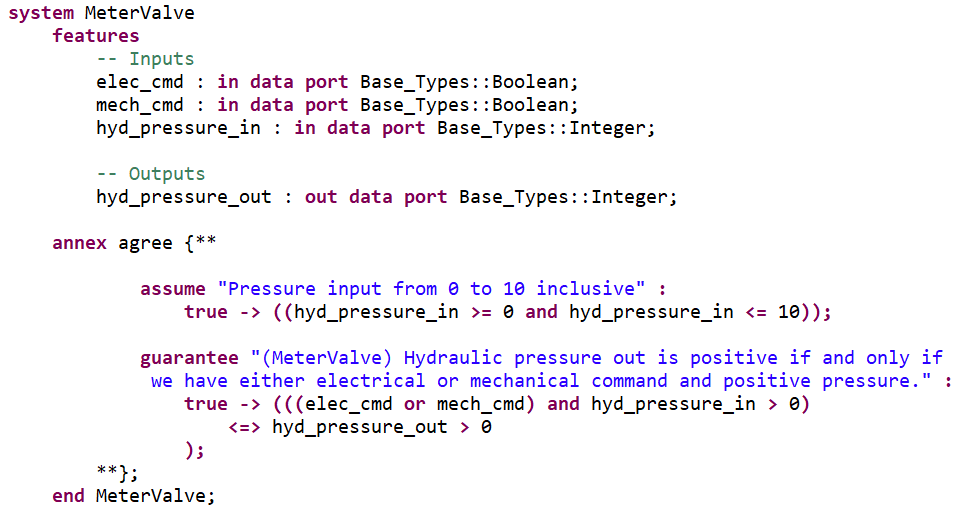
\includegraphics[width=0.8\textwidth]{images/metervalve.png}
%	\end{center}
%	\vspace{-0.3in}
%	\caption{AADL and AGREE Subcomponent: Meter Valve}
%	\label{fig:metervalve}
%	%\vspace{-0.2in}
%\end{figure} 

%If power and pressure are supplied while the wheel is rolling and ground speed is positive \textit{and the pedal is not pressed}, then braking force is zero. This dictates that there must be a subcomponent that shuts off the hydraulic pressure to the wheel brake when the pedal is not being pressed. In this architecture, this is the Meter Valve subcomponent. As shown in Figure \ref{fig:wbs}, the Meter Valve takes input from the Control System (the pedal command) and the Selector Valve (hydraulic pressure line). The contracts of this component support the inadvertent braking contract by stating that if the pedal is pressed and hydraulic pressure is supplied, then the hydraulic output of the Meter Valve is positive. The AADL and AGREE code is shown in Figure \ref{fig:metervalve}. 


\subsection{Nominal Model Analysis}
To illustrate nominal model analysis on the WBS, we first address the types of analysis that AGREE can perform. Using monolithic analysis, the contracts at the lower levels of the architecture are flattened and used in the proof of the top level safety properties of the system. Compositional analysis, on the other hand, will perform the proof layer by layer top down, essentially breaking the larger proof into subsets of smaller problems. For a more comprehensive description of these types of proofs and analyses, see research by Backus, et. al. \cite{cofer2012compositional,QFCS15:backes} 

The WBS has a total of 27 safety properties at the top level that are supported by subcomponent assumptions and guarantees. \danielle{Can provide a table of all these properties. There aren't 27 to be listed - a few are per wheel and ends up being around 12 properties. Is it worth making?} As a whole, the model consists of xx assumptions and xx guarantees. The analysis proves the safety properties at the top level in yy seconds for monolithic analysis and yy seconds for compositional analysis. \danielle{Can provide a figure of results in Agree if desired.} 

\subsection{Fault Model Analysis}
\danielle{Perhaps this paragraph can be reused in the modeling section? If not, delete. Now that the initial architecture is made in AADL and the nominal model proves using AGREE/JKind, the preliminary system safety assessment (PSSA) begins looking at the WBS subsystem and attempts to identify possible faults for the subcomponents using the hazard analysis as a guide. The PSSA assesses how failures can lead to the associated functional hazards of the aircraft FHA by identifying the elements and interactions that contribute to the relevant failure conditions. Utilizing the shared architectural and behavioral model, the assessment can focus on how various subcomponents can fail. These are then inserted into the model using the Safety Annex, and analysis can run. This analysis provides the necessary artifacts for the PSSA (e.g. fault trees, probabilities, etc.). }

In Section \ref{sec:fault_modeling}, the fault modeling process was discussed and now we focus on the analysis of that fault model. There are a variety of ways the model can be analyzed using the Safety Annex. 

\begin{itemize}
\item Maximum fault analysis performed monolithically: If the threshold for max no. of faults is set at $n$, the model checker attempts to prove the safety properties if any combination of $n$ faults are active in the system. If this cannot be done, it returns a counterexample showing a combination of active faults that result in a violation of the safety property. 

\item Maximum fault analysis performed compositionally: this analysis collects all fault combinations of cardinality up to and equal to $n$ for which when active, violate the safety properties in question. The user can then view the \textit{minimal cut sets} for any given property. 

\item Probabilistic fault analysis performed monolithically: Given a top level probability threshold and probabilities assigned per subcomponent fault, this analysis assumes independence between faults and determines if any combination of active faults with combined probabilities above the threshold will cause violation of the safety properties. If so, the counterexample reveals one such combination of faults. 

\item Probabilistic fault analysis performed compositionally: this analysis collects all such fault combinations such that their combined probabilities (assuming independence) are greater than or equal to the top level threshold and provides them to the user. 
\end{itemize}

\danielle{There are a couple of options for showing results of analysis run.} 

\danielle{ (1) Show all results from the 4 types of analysis. Pro: see all types of results, con: tedious and repedative.}

\danielle{ (2) Show results from one or two of the types. Pro: not so repedative, con: selective (won't show everything).}

\danielle{My suggestion is to pick two: one monolithic/comp and one max/prob. Since we have example regarding resiliant to one fault, perhaps monolithic probabilistic and compositional max 1 fault?}


As seen in \danielle{some discussion regarding the analysis runs...} one of the single points of failure in terms of the inadvertent braking safety property \danielle{reference figure or section that already talks about this property} is the pedal sensor component. In hopes to mitigate this point of failure, a number of options should be considered. One option is to add redundancy to the single sensor on the pedal by creating a sensor system and implementing a kind of voting strategy on multiple pedal sensors. Another approach is to create a monitor on the sensor. When the monitor detects anomolies in behavior of the sensor, it reports its validity to a higher level in the architecture. There are a variety of ways to mitigate this problem and we chose one such way to adjust the WBS in order to eliminate these sensor faults from the minimal cut sets. 

By creating a SensorSystem that contains three pedal sensors and a voter subcomponent, the rest of the system and contracts need not be changed. The inputs and outputs of the sensor system are identical to the sensor itself and thus makes for relatively easy implementation. A diagram of this additional WBS subsystem is shown in Figure X \danielle{If we want a diagram, I will happily make one.}.

The analysis was run again with these changes and show success in this particular single point of failure mitigation strategy. As can be seen through this single example, a system as large as the WBS would benefit from many iterations of this process. Furthermore, if the model is changed even slightly on the system development side, it would automatically be seen from the safety analysis perspective and any negative outcomes would be shown upon subsequent analysis runs. This effectively eliminates any miscommunications between the development and analysis teams and creates a new safeguard regarding model changes. 

\danielle{To end the section, summarize the key points: how we fit into the process and why it matters. Perhaps mention that this is only a small example of what can be modeled using the safety annex and for more information about modeling capabilities, look at the users guide.}


